% Created 2022-08-14 dom 18:21
% Intended LaTeX compiler: pdflatex
\documentclass[a4paper,12pt,twoside]{book}
\usepackage[utf8x]{inputenc}
\usepackage[T1]{fontenc}
\usepackage{graphicx}
\usepackage{grffile}
\usepackage{longtable}
\usepackage{wrapfig}
\usepackage{rotating}
\usepackage[normalem]{ulem}
\usepackage{amsmath}
\usepackage{textcomp}
\usepackage{amssymb}
\usepackage{capt-of}
\usepackage{hyperref}
\usepackage[spanish]{babel}
\usepackage{a4wide}
\usepackage{ucs}
\usepackage{amsthm}
\theoremstyle{teorema}
\newtheorem{teorema}{Teorema}[section]
\newtheorem{lema}[teorema]{Lema}
\newtheorem{corolario}[teorema]{Corolario}
\newtheorem{proposicion}[teorema]{Proposición}
\newtheorem{definicion}[teorema]{Definición}
\theoremstyle{remark}
\newtheorem{nota}{Nota}[section]
\newtheorem{ejemplo}[nota]{Ejemplo}
\newenvironment{demostracion}
{\noindent {\bf Demostración:}}
{\newline\mbox{ } \hfill $\square$}
\author{José A. Alonso}
\date{\today}
\title{Demostraciones en textos de matemáticas preuniversitarias}
\hypersetup{
 pdfauthor={José A. Alonso},
 pdftitle={Demostraciones en textos de matemáticas preuniversitarias},
 pdfkeywords={},
 pdfsubject={},
 pdfcreator={Emacs 27.1 (Org mode 9.4.6)},
 pdflang={Spanish}}
\begin{document}

\maketitle
\tableofcontents

\chapter*{Introducción}

Este libro es una recopilación de los teoremas que aparecen en los
libros de textos de matemáticas antes de la Universidad. Los textos
utilizados son los de \href{http://www.apuntesmareaverde.org.es/}{Apuntes Marea Verde}. La mayoría de los teoremas
están en los libros de textos sin demostraciones. En algunos teoremas he
puesto un enlace a su demostración en \href{https://proofwiki.org}{ProofWiki}.

\chapter{1° de ESO (12 años)}
\label{sec:org2e02aa1}

Del libro \href{http://www.apuntesmareaverde.org.es/grupos/mat/LOMLOE/1ESO/1ESO.pdf}{Matemáticasde 1º de ESO} de Apuntes Marea Verde.

\section{Números naturales. Divisibilidad.}
\label{sec:org07c9f04}

\subsection{Operaciones con números naturales}
\label{sec:orgd66bc4d}

\begin{itemize}
\item 25 Propiedad distributiva de la multiplicación respecto a la suma en los naturales.

\item 25 Propiedad conmutativa de la multiplicación

\item 25 Propiedad distributiva de la multiplicación respecto a la resta

\item 26 División de números naturales
\end{itemize}

\subsection{Divisibilidad}
\label{sec:orgaf52ecb}

\begin{itemize}
\item 31 Criterio de divisibilidad por 2: Un número entero es divisible por
2 cuando su última cifra es 0 o cifra par.

\item 31 Criterio de divisibilidad por 3: Un número entero es divisible por
3 cuando la suma de sus cifras es múltiplo de 3

\item 31 Criterio de divisibilidad por 4: Un número entero es divisible por
4 si el número formado por las dos últimas cifras del número
considerado es múltiplo de 4.

\item 31 Criterio de divisibilidad por 5: Un número entero es divisible por
5 cuando termina en 0 o en 5.

\item 32 Criterio de divisibilidad por 6: Un número entero es divisible por
6 cuando lo es a la vez por 2 y por 3.

\item 32 Criterio de divisibilidad por 9: Un número entero es divisible por
9 cuando la suma de sus cifras es 9 o múltiplo de 9.

\item 32 Criterio de divisibilidad por 10: Un número entero es divisible por
10 cuando termina en 0.

\item 32 Criterio de divisibilidad por 11: Un número entero es divisible por
11 cuando la diferencia entre la suma de las cifras que ocupan lugar
impar y la suma de las cifras que ocupan lugar par da 0 o múltiplo de
11
\end{itemize}

\subsection{Números primos}
\label{sec:orgf6b9faf}

\begin{itemize}
\item 38 Descomposición de un número natural en factores primos

\item 40 Cálculo del M.C.D. 1. Factorizamos los números. 2. Tomamos los
factores comunes a todos los números elevados el menor
exponente. 3. El producto de los factores considerados en el paso 2 es
el M.C.D.

\item 41 Cálculo del m.c.m. 1. Factorizamos los números 2. Tomamos los
factores comunes y no comunes elevados al mayor exponente. 3. El
producto de esos factores del paso anterior es el m.c.m.

\item 43 Si \(n\) es un número natural tal que \(2^{n}-1\) es primo, entonces
\(2^{n-1}(2^{n}-1)\) es un número perfecto.

\item 43 Hay infinitos números primos.
\end{itemize}

\section{Potencias y raíces}
\label{sec:org14c9e17}

\subsection{Potencias}
\label{sec:orge43704e}

\begin{itemize}
\item 53 Cero, elevado a cualquier exponente distinto de cero, es igual a 0.
\end{itemize}

\subsection{Operaciones con potencias}
\label{sec:org9c30541}

\begin{itemize}
\item 55 Producto de potencias de igual base: \(a^{n}a^{m} = a^{n+m}\)

\item 55 Cociente de potencias de igual base: \(\dfrac{a^{n}}{a^{m}} = a^{n-m}\)

\item 55 Elevar una potencia a otra potencia: \((a^{n})^{m} = a^{nm}\)

\item 56 Potencia de un producto: \((ab)^{n} = a^{n}b^{n}\)

\item 56 Potencia de un cociente: \(\left(\dfrac{a}{b}\right)^{n} = \dfrac{a^{n}}{b^{n}}\)
\end{itemize}

\subsection{Raíces}
\label{sec:org9964c77}

\begin{itemize}
\item 58 Introducir factores en el radical: Para introducir un número dentro
del radical se eleva el número al índice de la raíz y se multiplica
por el radicando.
\end{itemize}

\section{Fracciones}
\label{sec:orgb8a351a}

\subsection{Suma y resta de fracciones}
\label{sec:org97862c0}

\begin{itemize}
\item 93 Propiedades de la suma de fracciones.
\end{itemize}

\subsection{Producto y cociente de fracciones}
\label{sec:org7e03daf}

\begin{itemize}
\item 97 Propiedades del producto de fracciones.
\end{itemize}

\section{Figuras planas}
\label{sec:orgacaeee7}

\subsection{Circunferencia y círculo}
\label{sec:org99aa085}

\begin{itemize}
\item 184 Las mediatrices de todas las cuerdas de una circunferencia pasan
por el centro.

\item 184 La recta tangente a una circunferencia es perpendicular al radio
que pasa por el punto de tangencia.
\end{itemize}

\subsection{Triángulos}
\label{sec:org943837d}

\begin{itemize}
\item 185 La suma de los ángulos de un triángulo es 180°

\item 185 En un triángulo cualquier lado es siempre menor que la suma de los
otros dos y mayor que su diferencia.

\item 186 Las mediatrices de los tres lados del triángulo concurren en un
punto llamado circuncentro. Dicho punto equidista de los vértices y,
es el centro de la circunferencia circunscrita al triángulo.

\item 186 Las bisectrices de los ángulos de un triángulo concurren en un
punto llamado incentro. Dicho punto equidista de los lados del
triángulo y es el centro de la circunferencia inscrita en el
triángulo.

\item 187 Las tres alturas de un triángulo se cortan en el ortocentro.

\item 187 El punto de corte de las medianas se llama baricentro.

\item 188 Para comprobar que dos triángulos son iguales es suficiente
comprobar que se cumple uno de los tres criterios siguientes: 1º
Tienen los tres lados iguales. 2º Tienen dos lados iguales e igual el
ángulo comprendido entre ambos.  3º Tienen un lado igual adyacente a
dos ángulos también iguales.
\end{itemize}

\subsection{Cuadriláteros}
\label{sec:org71c42f3}

\begin{itemize}
\item 190 La suma de los ángulos de un cuadrilátero es 360°

\item 190 La diagonal de un paralelogramo lo divide en dos triángulos iguales.

\item 190 Las diagonales de un paralelogramo se cortan en el punto medio.

\item 190 Las diagonales tanto de un rombo como de un cuadrado, son perpendiculares.

\item 190 Al unir los puntos medios de un cuadrilátero, se forma un paralelogramo.
\end{itemize}

\section{Longitudes y áreas}
\label{sec:org023b04b}

\subsection{Perímetros y áreas de polígonos}
\label{sec:org45e9c6f}

\begin{itemize}
\item 201 El área de un cuadrado es el cuadrado de uno de sus lados.

\item 201 El área de un rectángulo es el producto de su base por su altura.

\item 202 Los paralelogramos tienen las siguientes propiedades:
\begin{itemize}
\item Los lados opuestos son iguales
\item Sus diagonales se cortan en sus puntos medios
\item Tienen un centro de simetría
\item Los romboides no tienen eje de simetría
\end{itemize}

\item 202 El área de un paralelogramo es el producto de su base por su
altura.

\item 202 El área de un triángulo es la mitad del área de un
paralelogramo.

\item 204 El área de un trapecio es igual a la mitad de la suma de sus
bases multiplicada por su altura.

\item 204 El área de un rombo es el producto de sus diagonales divididas entre 2

\item 205 El área de un romboide es el producto de su base y su altura.

\item 206 El área de un polígono regular es igual al semiperímetro por la
apotema.
\end{itemize}

\subsection{Perímetros y áreas de figuras circulares}
\label{sec:org2c569c4}

\begin{itemize}
\item 210 La longitud de la circunferencia es \(2 \pi r\).

\item 210 La longitud de un arco de circunferencia que abarca un ángulo de A
grados es \(\dfrac{2 \pi rA}{360}\).

\item 211 El área del círculo es igual al producto del número \(\pi·r^2\).

\item 212 El área de una corona circular es igual al área del círculo mayor
menos el área del círculo menor.

\item 212 El área de un sector circular que abarca un ángulo de \(n\) grados es igual a:
\(\dfrac{\pi r^2 n}{360}\).

\item 213 El área de un sector de corona circular formada por las circunferencias
concéntricas de radios \(r\) y \(R\) que abarca un ángulo de \(n\) grados es igual a:
\(\dfrac{\pi (R^2 - r^2)n}{360}\).
\end{itemize}

\section{Álgebra}
\label{sec:org69948a6}

\subsection{Ecuaciones de primer grado}
\label{sec:orgbb9c48f}

\begin{itemize}
\item 240 Si se suma o se resta a los dos miembros de una ecuación una misma
cantidad, se obtiene una ecuación equivalente.

\item 240 Si se multiplican o dividen los dos miembros de una ecuación por
una misma cantidad (distinta de cero), se obtiene una ecuación
equivalente.
\end{itemize}
\chapter{2° de ESO (13 años)}
\label{sec:org06e4bf7}

Del libro \href{http://www.apuntesmareaverde.org.es/grupos/mat/LOMLOE/2ESO/2ESO.pdf}{Matemáticasde 2º de ESO} de Apuntes marea Verde.

\section{Números}
\label{sec:org995799f}

\subsection{Operaciones}
\label{sec:org06f3f78}

\begin{itemize}
\item 35: Propiedades de la suma de fracciones: conmutativa, asociativa,
neutro y opuestos.

\item 35: Propiedades del producto de fracciones: conmutativa, asociativa,
neutro, opuestos de no nulos y distributiva respecto de sumas
\end{itemize}

\section{Potencias y raíces}
\label{sec:org000ac69}

\subsection{Potencias}
\label{sec:org8b3f9b0}

\begin{itemize}
\item 53 Una potencia de cualquier base distinta de cero elevada a cero es
igual a 1.

\item 53 Uno, elevado a cualquier exponente, es igual a 1.

\item 53 Cero, elevado a cualquier exponente distinto de cero, es igual a 0.

\item 54 La unidad seguida de ceros es igual a una potencia de 10.
\end{itemize}

\section{Operaciones con potencias y propiedades}
\label{sec:org2658969}

\begin{itemize}
\item 54 Para calcular el producto de dos o más potencias de la misma base,
se deja la misma base y se suman los exponentes.

\item 54 El cociente de potencias de igual base es igual a otra potencia de
la misma base y de exponente, la diferencia de los exponentes.

\item 54 Para elevar una potencia a otra potencia, se deja la misma base y
se multiplican los exponentes.

\item 55 La potencia de un producto es igual al producto de cada uno de los
factores elevados al mismo exponente.

\item 55 La potencia de un cociente es igual al cociente de cada uno de los
factores elevados al mismo exponente.

\item 55 Las potencias de base negativa y exponente par son números
positivos.

\item 55 Las potencias de base negativa y exponente impar son números
negativos.
\end{itemize}

\subsection{Raíces}
\label{sec:orgf430a44}

\begin{itemize}
\item 59 Para introducir un número dentro del radical se eleva el número al
índice de la raíz y se multiplica por el radicando.
\end{itemize}

\section{Divisibilidad}
\label{sec:org8f78c9c}

\subsection{Divisibilidad}
\label{sec:orgf60dfed}

\begin{itemize}
\item 71 Todo número tiene siempre como divisor a 1 y a sí mismo.

\item 72 Un número entero es divisible por 2 cuando su última cifra es 0 o
cifra par.

\item 72 Un número entero es divisible por 3 cuando la suma de sus cifras es
múltiplo de 3.

\item 72 Un número entero es divisible por 4 si el número formado por las
dos últimas cifras del número considerado es múltiplo de 4.

\item 73 Un número entero es divisible por 5 cuando termina en 0 o en 5.

\item 73 Un número entero es divisible por 6 cuando lo es a la vez por 2 y
por 3.

\item 73 Un número entero es divisible por 9 cuando la suma de sus cifras es
9 o múltiplo de 9

\item 73 Un número entero es divisible por 10 cuando termina en 0.

\item 73 Un número entero es divisible por 11 cuando la diferencia entre la
suma de las cifras que ocupan lugar impar y la suma de las cifras que
ocupan lugar par da 0 o múltiplo de 11.
\end{itemize}

\subsection{Números primos}
\label{sec:org3961afa}

\begin{itemize}
\item 79 Descomponer un número natural en factores primos es expresar dicho
número como un producto, donde todos sus factores son números primos.

\item 80 Cálculo del M.C.D.
\begin{itemize}
\item Factorizamos los números.
\item Tomamos los factores comunes a todos los números elevados el menor exponente.
\item El producto de los factores considerados en el paso 2 es el M.C.D
\end{itemize}

\item 81 Cálculo del m.c.m.
\begin{itemize}
\item Factorizamos los números
\item Tomamos los factores comunes y no comunes elevados al mayor exponente.
\item El producto de esos factores del paso anterior es el m.c.m.
\end{itemize}
\end{itemize}

\section{Longitudes y áreas. Semejanza}
\label{sec:orge2b42a1}

\subsection{Teorema de Pitágoras}
\label{sec:org88e6f67}

\begin{itemize}
\item 116 Teorema de Pitágoras: En un triángulo rectángulo, la hipotenusa al
cuadrado es igual a la suma de los cuadrados de los catetos.
\end{itemize}

\subsection{Semejanza}
\label{sec:org8a43adc}

\begin{itemize}
\item 118 Dos triángulos son semejantes si tienen todos los ángulos iguales
y los lados proporcionales.

\item 118 Dos triángulos son semejantes sí:
\begin{itemize}
\item Primero: Tienen dos ángulos iguales.
\item Segundo: Tienen los tres lados proporcionales.
\item Tercero: Tienen dos lados proporcionales y el ángulo que forman es igual.
\end{itemize}

\item 120 Teorema de Tales: Dadas dos rectas, y varias rectas paralelas
entre sí, que las cortan respectivamente en los puntos \(A\), \(B\), \(C\) y \(A’\),
\(B’\), \(C’\). Entonces los segmentos son proporcionales:
$$\dfrac{A'B'}{AB} = \dfrac{B'C'}{BC} = \dfrac{A'C'}{AC}$$

\item 121 Si la razón de semejanza entre las longitudes de una figura es \(k\),
entonces la razón entre sus áreas es \(k^2\).

\item 121 Si la razón de semejanza entre las longitudes de una figura es \(k\),
entonces la razón entre sus volúmenes es \(k^3\).
\end{itemize}

\section{Cuerpos geométrico. Volúmenes}
\label{sec:orgbddbd04}

\subsection{El espacio}
\label{sec:orgf2f239f}

\begin{itemize}
\item 145 Dos planos en el espacio son paralelos si no tienen ningún punto
en común, y son secantes si tienen una recta en común.

\item 146 Dos rectas en el espacio o son paralelas o se cortan o se cruzan.

\item 146 Una recta puede estar contenida en un plano o ser paralela al
plano o ser secante.
\end{itemize}

\subsection{Poliedros}
\label{sec:org8849062}

\begin{itemize}
\item 155 El volumen de un prisma es igual al producto del área de su base
por su altura.

\item 156 El volumen de una pirámide es un tercio del volumen del prisma que
tiene la misma base que la pirámide y la misma altura que ella.
\end{itemize}

\subsection{Cuerpos redondos}
\label{sec:org594b976}

\begin{itemize}
\item 160 La superficie del cilindro es \(2 \pi rh + 2 \pi r^2\).

\item 160 Superficie del cono = Área del sector circular + Área del círculo
= \(\pi rg + \pi r^2\).

\item 161 Superficie del tronco de cono = \(\pi (r+r')g + \pi r^2 + \pi r'^2\).

\item 161 Superficie de la esfera de radio \(r\) es igual a \(4 \pi r^2\).

\item 162 Volumen cilindro = \(\pi r^2 h\)

\item 162 Volumen cono = \(\dfrac{\pi r^2 h}{3}\)

\item 163 Volumen de la esfera = \(\dfrac{4 \pi r^3}{3}\).
\end{itemize}

\section{Álgebra}
\label{sec:org29d2310}

\subsection{Ecuaciones de 2º grado}
\label{sec:org7b338d2}

\begin{itemize}
\item 209 Resolución de ecuaciones de 2º grado \(ax^2+bx+c=0\)
$$x = \dfrac{-b \pm \sqrt{b^2 -4ac}}{2a}$$
\end{itemize}

\chapter{3° de ESO (14 años)}
\label{sec:orgfe136f6}

Del libro \href{http://www.apuntesmareaverde.org.es/grupos/mat/LOMLOE/3ESO/Tercero.pdf}{Matemáticas de 3º de ESO} de Apuntes marea Verde.

\section{Números racionales}
\label{sec:orgb1408a8}

\subsection{Recordatorio}
\label{sec:org13881f1}

\begin{itemize}
\item 8 Regla de los signos para la suma:
\begin{itemize}
\item La suma de 2 números positivos es positiva.
\item La suma de 2 números negativos es negativa.
\item La suma de un número positivo con otro negativo tendrá el signo del
mayor en valor absoluto.
\end{itemize}

\item 9 Regla de los signos para la multiplicación (y la división):
\begin{itemize}
\item Positivo x Positivo = Positivo
\item Positivo x Negativo = Negativo x Positivo = Negativo
\item Negativo x Negativo = Positivo.
\end{itemize}

\item 9
\begin{teorema}
\(0 \times x = 0\) para todo \(x\).
\end{teorema}

\begin{demostracion}
\begin{align*}
x \times 0 &= x \times (a - a)   \\
      &= x \times a - x \times a \\
      &= 0             \\
\end{align*}
\end{demostracion}

\item 10
\begin{teorema}
\((-1) \times (-1) = 1\)
\end{teorema}

\begin{demostracion}
\begin{align*}
 (-1) \times (-1) + (-1) &= (-1) \times (-1) + (-1) \times 1  \\
                    &= (-1) \times (-1 + 1) \\
                    &= (-1) \times 0 \\
                    &= 0
  \end{align*}
Por tanto, \((-1) \times (-1) = 1\).
\end{demostracion}
\end{itemize}

\section{Números racionales}
\label{sec:org3ea27f8}

\begin{itemize}
\item 13 Si \(a\) y \(b\) son positivos y \(a < b\), entonces \(\frac{1}{a} > \frac{1}{b}\).

\item 27 El número de cifras del periodo de \(\frac{1}{n}\) es menor o igual que \(n - 1\).

\item 27 En general \(\frac{1}{2^n \times 5^m}\) tiene expresión decimal exacta y el número
de cifras decimales es el máximo entre \(n\) y \(m\).

\item 27 Si en el denominador de una fracción irreducible aparecen factores
primos distintos de 2 y de 5 la expresión decimal será periódica.

\item 28 Para obtener la fracción generatriz se pone en el numerador el
número sin la coma y en el denominador la unidad seguida de tantos
ceros como cifras decimales tiene. Se simplifica la fracción.

\item 29 Para obtener la fracción generatriz de una expresión decimal
multiplicamos el número por la potencia de 10 necesaria para llevarnos
la coma al final del primer periodo, luego lo multiplicamos otra vez
para que la coma quede al principio del primer periodo.

\item 34 \(\frac{1}{2} + \frac{1}{4} + \frac{1}{16} + \frac{1}{32} + \cdots = 1\).
\end{itemize}

\section{Potencias y raíces}
\label{sec:org6e334a4}

\begin{itemize}
\item 59 \((a \times b \times c \times d)^n = a^n \times b^n \times c^n \times d^n\).

\item 59 \(\dfrac{c^m}{c^n} = c^{m-n}\)

\item 59 \((d^{m})^n = d^{mn}\)

\item 59 \(\left(\dfrac{a}{b}\right)^n = \dfrac{a^n}{b^n}\)

\item 59 \(a^{-n} = \dfrac{1}{a^n}\)
\end{itemize}

\section{Sucesiones}
\label{sec:orga82b128}

\subsection{Progresiones aritméticas}
\label{sec:orgba2b1c5}

\begin{itemize}
\item 71 El término general de una progresión aritmética es
$$a_{n} = a_{1} + (n - 1)d$$

\item 71 El término general de una progresión aritmética es
$$a_{n} = a_{k} + (n - k)d$$

\item 73
\begin{teorema}
En una progresión aritmética, la suma de dos términos equidistantes
es constante.  Es decir, si los subíndices naturales \(p\), \(q\), \(r\) y \(s\)
verifican que \(p + q = r + s\), entonces: \(a_{p} + a_{q} = a_{r} + a_{s}\).
\end{teorema}
\begin{demostracion}
\begin{align*}
 a_{p} + a_{q}  &= a_{1} + (p - 1)d + a_{1} + (q - 1)d \\
          &= 2a_{1} + (p + q - 2)d \\
          &= 2a_{1} + (r + s - 2)d \\
          &= a_{1} + (r - 1)d + a_{1} + (s - 1)d \\
          &= a_{r} + a_{s}
  \end{align*}
\end{demostracion}

\item 73
\begin{teorema}
La suma de los \(n\) primeros términos de una progresión aritmética es
\(\dfrac{a_1 + a_n}{2}\)
\end{teorema}
\begin{demostracion}
Sea \(S\) la suma de los \(n\) primeros términos. Entonces,
\begin{align*}
   S &= a_1 + a_2   + \dots + a_{n-1} + a_n \\
   S &= a_n + a_{n-1} + \dots + a_2   + a_1
\end{align*}

Sumando,
\begin{align*}
  2S &= (a_1 + a_n) + (a_2 + a_{n-1}) + \dots + (a_{n-1} + a_2) + (a_n + a_1) \\
     &= (a_1 + a_n) + (a_1 + a_n) + \dots + (a_1 + a_n) + (a_1 + a_n) \\
     &= (a_1 + a_n)n
\end{align*}

Por tanto,
$$S = \frac{a_1+a_n}{2}$$
\end{demostracion}
\end{itemize}

\subsection{Progresiones geométricas}
\label{sec:org70c0c26}

\begin{itemize}
\item 76 El término general de una progresión geométrica es
\(a_n = a_1 r^{n-1}\)

\item 78
\begin{teorema}
En una progresión geométrica, el producto de dos términos
equidistantes es constante. Es decir, si los subíndices naturales \(p\),
\(q\), \(t\) y \(s\) verifican que \(p + q = t + s\), entonces: \(a_p a_q = a_t a_s\).
\end{teorema}
\begin{demostracion}
\begin{align*}
 a_p a_q &= a_1 r^{p-1} a_1 r^{q-1} \\
         &= a_1 a_1 r^{p+q-2} \\
         &= a_1 a_1 r^{t+s-2} \\
         &= a_1 r^{t-1} a_1 r^{s-1} \\
         &= a_t a_s
\end{align*}
\end{demostracion}

\item 78
\begin{teorema}
El cuadrado del producto de los n primeros términos de una
progresión geométrica viene dado por \((a_1 a_n)^n\). \\
\end{teorema}
\begin{demostracion}
Sea \(P\) el producto de los \(n\) primeros términos de una progresión
geométrica. Entonces,
\begin{align*}
   P^2 &= (a_1 a_2 \dots a_{n-1} a_n) (a_n a_{n-1} \dots a_2 a_1) = \\
      &= (a_1 a_n) (a_2 a_{n-1}) \dots (a_{n-1} a_2) (a_n a_1) \\
      &= (a_1 a_n) (a_1  a_n) \dots (a_1 a_n) (a_1 a_n)  \\
      &= (a_1 a_n)^n
\end{align*}
\end{demostracion}

\item 79
\begin{teorema}
La suma de los \(n\) primeros términos de una progresión geométrica no
constante \(\dfrac{a_1(r^n - 1)}{r-1}\). \\
\end{teorema}
\begin{demostracion}
Se tiene
\begin{align*}
   S      &= a_1 + a_2 + \dots + a_{n-1} + a_n \\
\end{align*}
Multiplicando por \(r\)
\begin{align*}
   rS     &= r(a_1 + a_2 + \dots + a_{n-1} + a_n) \\
          &= r a_1 + r a_2 + \dots + r a_{n-1} + r a_n \\
          &= a_2   + a_3   + \dots + a_n + r a_n \\
\end{align*}
Restando
\begin{align*}
   rS - S &= r.a_n - a_1 \\
          &= r a_1 r^{n-1} - a_1 \\
          &= a_1(r^n -1)
\end{align*}
Luego,
   $$S = \frac{a_1(r^n - 1)}{r-1}$$.
\end{demostracion}

\item 81 La suma de un número ilimitado de términos de una progresión
geométrica sólo toma un valor finito si \(|r| < 1\), y entonces viene dada
por \(\frac{a_1}{1-r}\). En el resto de los casos, o vale infinito, o no existe pues
oscila.
\end{itemize}

\section{Expresiones algebraicas. Polinomios}
\label{sec:org00b587a}

\subsection{Polinomios. Suma y producto}
\label{sec:org7bafc7a}

\begin{itemize}
\item 100 Propiedades de la suma de polinomios: conmutativa, asociativa,
neutro y opuestos.

\item 104 Propiedades del producto de polinomios: conmutativa, asociativa,
neutro y distributiva.
\end{itemize}

\subsection{División de polinomios}
\label{sec:org632cab7}

\begin{itemize}
\item 107 Dados dos polinomios \(p(x)\) y \(q(x)\), la división de \(p(x)\),
polinomio dividendo, entre \(q(x)\), polinomio divisor, nos
proporcionará otros dos polinomios, el polinomio cociente \(c(x)\) y el
polinomio resto \(r(x)\).  Además, su grado deberá ser menor que el
grado del polinomio divisor. La relación entre los cuatro es
\(p(x) = q(x)c(x) + r (x)\).
\end{itemize}

\subsection{Igualdades notables}
\label{sec:org21b73d4}

\begin{itemize}
\item 111 Potencias de un binomio:
\begin{itemize}
\item \((a + b)^{2} = a^{2} + 2ab + b^{2}\)
\item \((a - b)^{2} = a^{2} - 2ab + b^{2}\)
\item \((a + b)^{3} = a^{3} + 3a^{2}b + 3ab^{2} + b^{3}\)
\item \((a - b)^{3} = a^{3} - 3a^{2}b + 3ab^{2} - b^{3}\)
\end{itemize}

\item 112 Suma por diferencia: \((a + b)(a - b) = a^{2} - b^{2}\).
\end{itemize}

\section{Ecuaciones y sistemas}
\label{sec:orgf013fa7}

\subsection{Ecuaciones de segundo grado}
\label{sec:org85954b2}

\begin{itemize}
\item 132
\begin{teorema}
La suma de la raíces de la ecuación \(x^{2} + bx + c = 0\)  es \(-b\) y su
producto es \(c\).
\end{teorema}
\begin{demostracion}
Sean \(x_1\) y \(x_2\) la raíces de \(x^{2} + bx + c = 0\). Entonces,
\begin{align*}
   x^{2} + bx + c &= (x - x_1)(x - x_2) \\
               &= x^{2} - (x_1 + x_2)x + x_1 x_2
\end{align*}
Por tanto, \(x_1 + x_2 = -b\) y \(x_1 x_2 = c\).
\end{demostracion}

\item 132
\begin{teorema}
La soluciones de \(ax^{2} + bx + c = 0\), con \(a \ne 0\), son
$$\frac{-b \pm \sqrt{b^{2}-4ac}}{2a}$$
\end{teorema}
\begin{demostracion}
\begin{align*}
   & ax^{2} + bx + c = 0 \\
 & ax^{2} + bx = -c \\
 & 4a(ax^{2} + bx) = -4ac  \\
 & 4a(ax^{2} + bx) + b^{2} = -4ac + b^{2}  \\
 & 4a^{2}x^{2} + 4abx + b^{2} = -4ac + b^{2}  \\
 & (2ax + b)^{2} = -4ac + b^{2}  \\
 & 2ax + b = \pm \sqrt{b^{2}-4ac} \\
 & x = \frac{-b \pm \sqrt{b^{2}-4ac}}{2a}
\end{align*}
\end{demostracion}
\end{itemize}

\section{Geometría en el plano}
\label{sec:orge14b778}

\subsection{Lugares geométricos}
\label{sec:orgd455b4d}

\begin{itemize}
\item 174 La circunferencia es el lugar geométrico de los puntos del plano
cuya distancia a un punto del mismo (el centro) es un valor
determinado (el radio).

\item 174 La mediatriz de un segmento es el lugar geométrico de los puntos
del plano que equidistan de los extremos del mismo.

\item 174 La mediatriz es una recta perpendicular al segmento y pasa por el
punto medio del mismo.

\item 174 Dado un ángulo delimitado por dos rectas, la bisectriz del ángulo
es el lugar geométrico de los puntos del plano que equidistan de las
mismas.

\item 174 La bisectriz pasa por el vértice del ángulo y divide a éste en dos
ángulos iguales.
\end{itemize}

\subsection{Ángulos, longitudes y áreas}
\label{sec:org9f3d6a5}

\begin{itemize}
\item 183 Teorema de Pitágoras: En un triángulo rectángulo, la hipotenusa al
cuadrado es igual a la suma de los cuadrados de los catetos.

\item 185 La suma de los ángulos interiores de un triángulo es \(180^{\circ}\)

\item 185 La suma de los ángulos interiores de un polígono de \(n\) lados es
\((n - 2) 180^{\circ}\)

\item 187 Un ángulo inscrito mide la mitad que un ángulo central que abarca
el mismo arco de circunferencia. \\
Demostración gráfica.

\item 188 En cualquier triángulo rectángulo el circuncentro está en el punto
medio de la hipotenusa.

\item 188 Un ángulo inscrito en la circunferencia que abarca un diámetro es
un ángulo recto.
\end{itemize}

\section{Revisión de Geometría en el espacio}
\label{sec:orgf3fd5e4}

\begin{itemize}
\item 252 Teorema de Euler: en todo poliedro convexo el número de caras más
el número de vértices coincide con el número de aristas más 2.

\item 256 Teorema de Pitágoras en el espacio: La diagonal de un ortoedro al
cuadrado coincide con la suma de los cuadrados de sus aristas.

\item 260 El área lateral de una pirámide regular es la mitad del producto
del perímetro de la base por la apotema.
\end{itemize}

\chapter{4° de ESO (15 años)}
\label{sec:org498b279}

Del libro \href{http://www.apuntesmareaverde.org.es/grupos/mat/LOMLOE/4B/CuartoB.pdf}{Matemáticas de 4º de ESO}º de Apuntes marea Verde.

\section{Números reales}
\label{sec:orgad6805a}

\subsection{Números racionales e irracionales}
\label{sec:org75c7893}

\begin{itemize}
\item 9
\begin{teorema}
\(\sqrt{2}\) no es un número racional.
\end{teorema}
\begin{demostracion}
Demostración (por reducción al absurdo)

Supongamos que \(\sqrt{2}\) es racional. Entonces, se puede escribir como
una fracción irreducible
   $$\sqrt{2} = \frac{a}{b}$$
Por tanto,
\begin{align*}
   & 2 = \frac{a²}{b²} \\
   & a² = 2b²
  \end{align*}
Luego \(a²\) es par y por lo tanto \(a\) también lo es (el cuadrado de un
número impar es siempre impar). Ponemos \(a = 2k\) y sustituimos:
\begin{align*}
   & (2k)² = 2b² \\
   & 4k² = 2b² \\
   & 2k² = b²
\end{align*}
Luego \(b²\) es par y por tanto \(b\) también lo será. En definitiva: \(a\) y \(b\)
son los 2 números pares que es una contradicción con el que
\(\frac{a}{b}\) es  irreducible.
\end{demostracion}

\item 11 \(\sqrt{7}\) es irracional.

\item 14 En cada suma o resta el error absoluto es la suma de los errores
absolutos.

\item 14 Los errores relativos se suman al multiplicar dos números.

\item 32 \(e\) es límite de la sucesión \(\left(1 + \frac{1}{n}\right)^n\)
\item 33 \(e = 1 + \frac{1}{1!} + \frac{1}{2!} + \frac{1}{3!} + \dots\)
\end{itemize}

\subsection{Densidad de los números reales}
\label{sec:org37c3ecc}

\begin{itemize}
\item 16
\begin{teorema}
Los números reales son densos, es decir, entre cada dos números
reales hay infinitos números en medio.
\end{teorema}
\begin{demostracion}
Sea a y b dos números reales tales que \(a < b\). Entonces, se consideran
\begin{align*}
  c &= \frac{a+b}{2} \\
  d &= \frac{a+c}{2}
\end{align*}
y se tiene
   $$a < d < c < b$$
Repitiendo el proceso se obtienen infinitos números entre \(a\) y \(b\).
\end{demostracion}

\item 16 Los racionales son también densos.
\end{itemize}

\section{Potencias y raíces}
\label{sec:org718e45c}

\subsection{Logaritmos}
\label{sec:org71a40de}

\begin{itemize}
\item 48
\begin{teorema}
El logaritmo de 1 es cero (en cualquier base)
\end{teorema}
\begin{demostracion}
Como \(a^0 = 1\), por definición de logaritmo, tenemos que \(\log_{a} 1 = 0\).
\end{demostracion}

\item 48
\begin{teorema}
Si \(a > 0\), entonces \(\log_{a} a = 1\).
\end{teorema}
\begin{demostracion}
Como \(a^1 = a\), por definición de logaritmo, tenemos que \(\log_{a} a = 1\).
\end{demostracion}
\end{itemize}


\begin{itemize}
\item 48 Solo tienen logaritmos los números positivos.

\item 48
\begin{teorema}
\(\log_{a} (x y) = \log_{a} x + \log_{a} y\).
\end{teorema}
\begin{demostracion}
Sean \(A = \log_{a} x\) y \(B = \log_{a} y\). Por definición de logaritmos sabemos
que:
\begin{align*}
   a^{A} &= x \\
   a^{B} &= y
\end{align*}

Multiplicando:
\begin{align*}
   x y &= a^A   a^B \\
       &= a^{A+B}
\end{align*}
Luego,
\begin{align*}
 \log_{a} (x y) &= A + B \\
             &= \log_{a} x + \log_{a} y.
\end{align*}
\end{demostracion}

\item 48
\begin{teorema}
El logaritmo de un cociente es igual al logaritmo del dividendo
menos el logaritmo del divisor.
\end{teorema}
\begin{demostracion}
Sean \(A = \log_{a} x\) y \(B = \log_{a} y\). Por definición de logaritmos sabemos
que:
\begin{align*}
   a^A &= x \\
   a^B &= y
\end{align*}
Dividiendo
\begin{align*}
  \frac{x}{y} &= \frac{a^A}{a^B} \\
              &= a^{A-B}
  \end{align*}
Luego,
\begin{align*}
   \log_{a} (\frac{x}{y}) &= A - B \\
                      &= \log_{a} x - \log_{a} y
\end{align*}
\end{demostracion}

\item 48
\begin{teorema}
El logaritmo de una potencia es igual al exponente multiplicado por
el logaritmo de la base de la potencia.
\end{teorema}
\begin{demostracion}
Sea \(A = \log_{a} x\). Por definición de logaritmos sabemos que:
   $$a^A = x$$
Por tanto,
\begin{align*}
   x^y &= (a^A)^y \\
      &= a^{Ay}
\end{align*}
Luego,
\begin{align*}
   \log_{a} (x^y) &= y A \\
             &= y \log_{a} x
\end{align*}
\end{demostracion}

\item 48
\begin{teorema}
\(\log_{a} \sqrt[n]{b} = \dfrac{\log_a}{n}\).
\end{teorema}
\begin{demostracion}
\begin{align*}
 \log_{a} \sqrt[n]{b} &= \log_{a} {b}^{\frac{1}{n}} \\
                   &= \dfrac{\log_a}{n}
\end{align*}
\end{demostracion}

\item 49 Cambio de base:
$$\log_a x = \dfrac{\log_{b} x}{\log_{b} a}$$
\end{itemize}

\section{Sumas y productos de polinomios.}
\label{sec:org6f8a06b}

\begin{itemize}
\item 65 Propiedades de la suma de polinomios.

\item 68 Propiedades del producto de polinomios.
\end{itemize}

\section{División de polinomios}
\label{sec:org7406637}

\begin{itemize}
\item Existencia de la división.
\end{itemize}

\section{Raíces de un polinomio}
\label{sec:org23e0797}

\begin{itemize}
\item 78
\begin{teorema}
Si un número real \(\alpha\) es una raíz del polinomio \(p(x)\), entonces el
polinomio \(x - \alpha\) divide a \(p(x)\).
\end{teorema}
\begin{demostracion}
Dividiendo \(p(x)\) entre \(x - \alpha\) se tiene
   $$p(x) = (x - \alpha) c(x) + r (x)$$
Como el polinomio divisor, \(x - \alpha\), es de grado 1, y el polinomio resto
ha de ser de inferior grado, se deduce que el resto anterior es un
número real. Luego,
   $$p(x) = (x - \alpha) c(x) + \beta$$
El polinomio de la izquierda, \(p(x)\), es idéntico al de la derecha. Por
esa razón, al evaluarlos en cierto número real obtendremos el mismo
valor. Procedamos a particularizarlos para \(x = \alpha\)  Al ser \(\alpha\) raíz de
\(p(x)\), \(p(\alpha) = 0\). Esto nos lleva a
\begin{align*}
   0 &= p(\alpha) \\
     &= (\alpha - \alpha) c(\alpha) + \beta \\
     &= 0 c(\alpha) + \beta \\
     &= 0 + \beta \\
     &= \beta
\end{align*}
y, así, el resto es \(0\), y \(p(x) = (x - \alpha)c(x)\).
\end{demostracion}

\item 79
\begin{teorema}
Si un polinomio \(p(x)\) admite una descomposición factorial de la forma
\(p(x) = (x - \alpha) \times c(x)\) para cierto polinomio \(c(x)\) y
cierto número real \(\alpha\), entonces el número \(\alpha\) es una raíz
del polinomio \(p(x)\).
\end{teorema}
\begin{demostracion}
Basta evaluar \(p\) en \(x = \alpha\):
\begin{align*}
   p(\alpha) &= (\alpha - \alpha) \times c(\alpha) \\
             &= 0 \times c(\alpha) \\
             &= 0
\end{align*}
\end{demostracion}

\item 79 (\href{https://proofwiki.org/wiki/Condition\_for\_Linear\_Divisor\_of\_Polynomial}{Condition for linear divisor of polynomial} en ProofWiki)
\begin{teorema}
Teorema del factor. Un número real \(\alpha\) es raíz de un polinomio
\(p(x)\) si y solo si el polinomio \(x - \alpha\) divide a \(p(x)\); es
decir, si y solo si el polinomio \(p(x)\) admite una descomposición
factorial de la forma \(p(x) = (x - \alpha) \times c(x)\).
\end{teorema}
\begin{demostracion}
Es consecuencia de las dos propiedades anteriores.
\end{demostracion}

\item 80 Todo polinomio de grado \(n\) tiene a lo sumo \(n\) raíces reales, alguna
de las cuales puede aparecer repetida entre esos no más de \(n\) números
reales.

\item 81 Todo polinomio de grado impar posee, al menos, una raíz real.
\end{itemize}

\subsection{Regla de Ruffini}
\label{sec:orgf3940bd}

\begin{itemize}
\item 84 [Teorema del resto]. El valor numérico que adopta un polinomio \(p(x)\)
en \(x = \alpha\) coincide con el resto que aparece al dividir \(p(x)\)
entre \(x - \alpha\). (\href{https://proofwiki.org/wiki/Little\_B\%C3\%A9zout\_Theorem}{Little Bézout theorem} en ProofWiki).
\end{itemize}

\subsection{Cálculo de las raíces de un polinomio}
\label{sec:org4a90c09}

\begin{itemize}
\item 86
\begin{teorema}
Dado un polinomio cualquiera cuyos coeficientes son todos números
enteros, sus raíces enteras, si las tuviera, se encuentran
necesariamente entre los divisores enteros de su término
independiente.
\end{teorema}
\begin{demostracion}
Supongamos que el número entero \(\alpha\) es una raíz del polinomio
$$a_{n}x^{n} + a_{n-1}x^{n-1} + \cdots + a_{2}x^{2} + a_{1}x + a_{0}$$
Tal número debe anularlo:
\begin{align*}
&a_{n}\alpha^{n} + a_{n-1}\alpha^{n-1} + \cdots + a_{2}\alpha^{2} + a_{1}\alpha + a_{0} \\
&a_{n}\alpha^{n} + a_{n-1}\alpha^{n-1} + \cdots + a_{2}\alpha^{2} + a_{1}\alpha = -a_{0} \\
&\alpha(a_{n}\alpha^{n-1} + a_{n-1}\alpha^{n-2} + \cdots + a_{2}\alpha + a_{1}) = -a_{0} \\
&a_{n}\alpha^{n-1} + a_{n-1}\alpha^{n-2} + \cdots + a_{2}\alpha + a_{1} = -\frac{a_{0}}{\alpha} \\
\end{align*}
En la última igualdad, el número del lado izquierdo es entero, porque
está expresado como una suma de productos de números enteros. Por
ello, el número del lado derecho, \(-\frac{a_{0}}{\alpha}\), también es
entero y, por tanto, \(\alpha\) es un divisor de \(a_{0}\).
\end{demostracion}

\item 87 Dado un polinomio cualquiera cuyos coeficientes son todos números
enteros, sus raíces racionales, si las tuviera, necesariamente tienen
por numerador algún divisor del término independiente y por
denominador algún divisor del coeficiente del término de mayor grado.
\end{itemize}

\subsection{Productos notables de polinomios}
\label{sec:org0a661c7}

\begin{itemize}
\item 89 Potencias de un binomio:
\begin{itemize}
\item \((a + b)^{2} = a^{2} + 2ab+ b^{2}\)
\item \((a - b)^{2} = a^{2} - 2ab+ b^{2}\)
\item \((a + b)^{3} = a^{3} + 3a^{2}b + 3ab^{2} + b^{3}\)
\item \((a - b)^{3} = a^{3} - 3a^{2}b + 3ab^{2} - b^{3}\)
\end{itemize}

\item 90 Suma por diferencia: \((a + b)(a - b) = a^{2} - b^{2}\).
\end{itemize}

\section{Ecuaciones y sistemas}
\label{sec:org460cbd4}

\begin{itemize}
\item Igual que en 3º
\end{itemize}

\section{Inecuaciones}
\label{sec:orgf92cca1}

\begin{itemize}
\item 149 Propiedades de las desigualdades
\begin{itemize}
\item \(a < b ⟹ a + c < b + c\)
\item Si \(c > 0\), entonces, \(a < b ⟹ ac < bc\)
\item Si \(c < 0\), entonces, \(a < b ⟹ a · c > b · c\)
\end{itemize}
\end{itemize}

\section{Semejanza}
\label{sec:orgd79c372}

\subsection{Teorema de Tales}
\label{sec:org070749d}

\begin{itemize}
\item 189 Demostración de teorema de Tales.
\end{itemize}

\subsection{Teorema de la altura y del cateto}
\label{sec:org2c59b87}

\begin{itemize}
\item 189 Teorema de la altura: En un triángulo rectángulo la altura es
media proporcional entre los segmentos en los que divide a la
hipotenusa.

\item 189 Teorema del cateto: En un triángulo rectángulo un cateto es media
proporcional entre la hipotenusa y su proyección sobre ella.
\end{itemize}

\section{Trigonometría}
\label{sec:orgd1bbe63}

\subsection{Relaciones fundamentales}
\label{sec:org6913324}

\begin{itemize}
\item 213
\begin{teorema}
Primera relación fundamental: \(\sen^{2}\alpha + \cos^{2} \alpha = 1\).
\end{teorema}
\begin{demostracion}
Por el teorema de Pitágoras,
$$a^{2} = b^{2} + c^{2}$$
Dividiendo por \(a^{2}\)
\begin{align*}
  1 &= \frac{a^{2}}{a^{2}} \\
    &= \frac{b^{2}}{a^{2}} + \frac{c^{2}}{a^{2}} \\
    &= \sen^{2} \alpha + \cos^{2} \alpha
\end{align*}
\end{demostracion}

\item 213
\begin{teorema}
Segunda relación fundamental: \(\tan \alpha = \dfrac{\sen \alpha}{\cos \alpha}\)
\end{teorema}
\begin{demostracion}
\begin{align*}
\dfrac{sen \alpha}{cos \alpha}
  &= \dfrac{\frac{b}{a}}{\frac{c}{a}} \\
  &= \dfrac{b}{c} \\
  &= \tan \alpha
\end{align*}
\end{demostracion}

\item 214
\begin{teorema}
\(\sec^{2} \alpha = 1 + \tan^{2} \alpha\)
\end{teorema}
\begin{demostracion}
\begin{align*}
\sec^{2} \alpha
  &= \dfrac{1}{cos^{2} \alpha} \\
  &= \dfrac{\sen^{2} \alpha + \cos^{2} \alpha}{\cos^{2} \alpha} \\
  &= \tan^{2} \alpha + 1
\end{align*}
\end{demostracion}

\item 214
\begin{teorema}
\(\cosec^{2} \alpha = 1 + \cot^{2} \alpha\)
\end{teorema}
\begin{demostracion}
\begin{align*}
\cosec^{2} \alpha
  &= \dfrac{1}{\sen^{2} \alpha} \\
  &= \dfrac{\sen^{2} \alpha + \cos^{2} \alpha}{\sen^{2} \alpha} \\
  &= 1 + \cot^{2} \alpha
\end{align*}
\end{demostracion}
\end{itemize}

\subsection{Razones trigonométricas de 30⁰, 45⁰ y 60⁰.}
\label{sec:orga33da24}

\begin{itemize}
\item 213 Razones trigonométricas de 60\textsuperscript{0}
\begin{itemize}
\item \(\sen 60^{0} = \dfrac{\sqrt{3}}{2}\)
\item \(\cos 60^{0} = \dfrac{1}{2}\)
\item \(\tan 60^{0} = \sqrt{3}\)
\end{itemize}

\item 213 Razones trigonométricas de 30º
\begin{itemize}
\item \(\sen 30^{0} = \dfrac{1}{2}\)
\item \(\cos 30^{0} = \dfrac{\sqrt{3}}{2}\)
\item \(\tan 30^{0} = \dfrac{\sqrt{3}}{3}\)
\end{itemize}

\item 213 Razones trigonométricas de 45º
\begin{itemize}
\item \(\sen 45^{0} = \dfrac{\sqrt{2}}{2}\)
\item \(\cos 45^{0} = \dfrac{\sqrt{2}}{2}\)
\item \(\tan 45^{0} = 1\)
\end{itemize}
\end{itemize}

\subsection{Teorema de los senos}
\label{sec:org0cc6ae4}

\begin{itemize}
\item 223
\begin{teorema}
En todo triángulo se cumple que los lados son proporcionales a los
senos de los ángulos opuestos.
\end{teorema}
\begin{demostracion}
Demostración gráfica.
\end{demostracion}
\end{itemize}

\subsection{Teorema de los cosenos}
\label{sec:org1968256}

\begin{itemize}
\item 224 En un triángulo ABC cualquiera se cumple que:
\begin{itemize}
\item \(a^{2} = b^{2} + c^{2} - 2bc \cos A\)
\item \(b^{2} = a^{2} + c^{2} - 2ac \cos B\)
\item \(c^{2} = a^{2} + b^{2} - 2ab \cos C\)
\end{itemize}
\end{itemize}

\section{Geometría}
\label{sec:org133ccf8}

\begin{itemize}
\item 251 Las rectas \(ax + by = c\) y \(a'x + b'y = c'\) son paralelas si
\(\dfrac{a}{a'} = \dfrac{b}{b'} \neq \dfrac{c}{c'}\).

\item 251 Las rectas \(\mathbf{OX} = \mathbf{OA} + t\mathbf{v}\) y \(\mathbf{OX} = \mathbf{OB} + t\mathbf{w}\) son paralelas si \(\mathbf{v} = k\mathbf{w}\)

\item 251 Las rectas \(ax + by = c\) y \(a'x + b'y = c'\) son perpendiculares si
\(a·a' + b·b' = 0\).

\item 251 Las rectas \(\mathbf{OX} = \mathbf{OA} + t\mathbf{v}\) y \(\mathbf{OX} = \mathbf{OB} + t\mathbf{w}\) son perpendiculares si \(v_{1}w_{1} + v_{2}w_{2} = 0\).
\end{itemize}

\section{Combinatoria}
\label{sec:org0932fd6}

\subsection{Permutaciones}
\label{sec:org33cb14c}

\begin{itemize}
\item 423 El número de permutaciones de un conjunto de \(n\) elementos es \(n!\).
\end{itemize}

\subsection{Variaciones}
\label{sec:org3917306}

\begin{itemize}
\item 429 El número de variaciones con repetición de \(m\) elementos tomados
de \(n\) en \(n\) es \(m^{n}\).

\item 429 El número de variaciones sin repetición de \(m\) elementos tomados
de \(n\) en \(n\) es \(m(m-1) \dots (m-n+1)\)
\end{itemize}

\subsection{Combinaciones}
\label{sec:orga6707c2}

\begin{itemize}
\item 433 El número de variaciones sin repetición de \(m\) elementos tomados
de \(n\) en \(n\) es \(\dfrac{m!}{(m-n)!n!}\)

\item 434
\begin{teorema}
\(\dbinom{m}{0} = 1\).
\end{teorema}
\begin{demostracion}
\begin{align*}
 \binom{m}{0} &= \dfrac{m!}{(m-0)!0!} \\
              &= \dfrac{m!}{m!1}      \\
              &= 1
\end{align*}
\end{demostracion}

\item 434
\begin{teorema}
\(\dbinom{m}{m} = 1\).
\end{teorema}
\begin{demostracion}
\begin{align*}
 \binom{m}{0} &= \dfrac{m!}{(m-m)!m!} \\
              &= \dfrac{m!}{0!m!}     \\
              &= \dfrac{1}{0!m!}      \\
              &= 1
\end{align*}
\end{demostracion}

\item 434
\begin{teorema}
\(\dbinom{m}{1} = m\).
\end{teorema}
\begin{demostracion}
\begin{align*}
 \binom{m}{0} &= \dfrac{m!}{(m-1)!1!} \\
              &= m
\end{align*}
\end{demostracion}
\end{itemize}


\begin{itemize}
\item 434
\begin{teorema}
\(\dbinom{m}{n} = \dbinom{m}{m-n}\).
\end{teorema}
\begin{demostracion}
\begin{align*}
 \binom{m}{n} &= \dfrac{m!}{(m-n)!n!} \\
              &= \dfrac{m!}{n!(m-n)!} \\
              &= \dfrac{m!}{(m-(m-n)!(m-n)!} \\
              &= \binom{m}{m-n}
\end{align*}
\end{demostracion}

\item 435
\begin{teorema}
\(\dbinom{m}{n} = \dbinom{m-1}{n} + \dbinom{m-1}{n-1}\).
\end{teorema}
\begin{demostracion}
\begin{align*}
 \binom{m-1}{n} + \binom{m-1}{n-1}
 &= \dfrac{(m-1)!}{((m-1)-n)!n!} + \dfrac{(m-1)!}{((m-1)-(n-1))!(n-1)!} \\
 &= \dfrac{(m-1)!}{(m-n-1)!n!} + \dfrac{(m-1)!}{(m-n)!(n-1)!} \\
 &= \dfrac{(m-1)!}{(m-n-1)!n(n-1)!} + \dfrac{(m-1)!}{(m-n)(m-n-1)!(n-1)!} \\
 &= \dfrac{(m-n)(m-1)!}{(m-n)(m-n-1)!n(n-1)!} + \dfrac{n(m-1)!}{n(m-n)(m-n-1)!(n-1)!} \\
 &= \dfrac{(m-n)(m-1)!}{(m-n)!n!} + \dfrac{n(m-1)!}{(m-n)!n!} \\
 &= \dfrac{(m-n)(m-1)! + n(m-1)!}{(m-n)!n!} \\
 &= \dfrac{(m-n+n)(m-1)!}{(m-n)!n!} \\
 &= \dfrac{m(m-1)!}{(m-n)!n!} \\
 &= \dfrac{m!}{(m-n)!n!} \\
 &= \binom{m}{n}
\end{align*}
\end{demostracion}
\end{itemize}

\subsection{Binomio de Newton}
\label{sec:org369ccf9}

\begin{itemize}
\item 440 \((a+b)^{n} = \binom{n}{0}a^{0} + \binom{n}{1}a^{n-1}b + \binom{n}{2}a^{n-2}b^{2} + \cdots + \binom{n}{n-1}a^{}b^{n-1} + \binom{n}{n}^{}b^{n}\)

\item 440 \((a-b)^{n} = \binom{n}{0}a^{0} - \binom{n}{1}a^{n-1}b + \binom{n}{2}a^{n-2}b^{2} + \cdots + (-1)^{n}\binom{n}{n}^{}b^{n}\)
\end{itemize}


\subsection{Permutaciones con repetición}
\label{sec:orga32cb52}

\begin{itemize}
\item 443 El número de permutaciones de 8 elementos de los que uno se repite
3 veces y otro 2 es \(\dfrac{8!}{2!3!}\).
\end{itemize}

\subsection{Combinaciones con repetición}
\label{sec:org3e2de91}

\begin{itemize}
\item 444 El número de combinaciones con repetición de m elementos tomados
de n en n es \(\binom{m+n-1}{n}\).
\end{itemize}

\section{Azar y probabilidad}
\label{sec:org0c2cf23}

\subsection{Probabilidad}
\label{sec:org01d7d49}

\begin{itemize}
\item 468 Probabilidad del suceso contrario: \(P(S^{C}) = 1 - P(S)\).

\item 468 Si \(A\) y \(B\) son independientes, \(P(A \cap B) = P(A) \cdot P(B)\).
\end{itemize}

\subsection{Probabilidad condicionada}
\label{sec:org8e0c453}

\begin{itemize}
\item 474 La probabilidad de verificación del suceso \(A\) condicionada a la
verificación del suceso \(B\) es \(P(A/B) = \dfrac{P(A \cap B)}{P(B)}\).
\end{itemize}

\chapter{1° de Bachillerato (16 años)}
\label{sec:org916f6ec}

Del libro \href{http://www.apuntesmareaverde.org.es/grupos/mat/LOMLOE/Bachillerato/Matematicas\_I.pdf}{Matemáticas I (1º de Bachillerato)} de Apuntes marea Verde.

\section{Números reales y complejos}
\label{sec:org3483780}

\subsection{Valor absoluto}
\label{sec:orga32ae41}

\begin{itemize}
\item 10 No negatividad: \(|a| \geq 0\).

\item 10
\begin{teorema}
Simetría: \(|a| = |-a|\).
\end{teorema}
\begin{demostracion}
Si \(a > 0\), entonces
\begin{align*}
|a| &= a \\
    &= -(-a) \\
    &= |-a|
\end{align*}

Si \(a = 0\), entonces
\begin{align*}
    |a| &= |0| \\
        &= |-0| \\
        &= |-a|
\end{align*}

Si \(a < 0\), entonces
\begin{align*}
|a| &= -a \\
    &= |-a|
\end{align*}
\end{demostracion}

\item 10 Definición positiva: Si \(|a| = 0\), entonces \(a = 0\).

\item 10 Valor absoluto y producto: \(|a \times b| = |a| \times |b|\).

\item 10 Desigualdad triangular: \(|a + b| \leq |a| + |b|\).
\end{itemize}

\subsection{Distancia en la recta real}
\label{sec:orge24d0ab}

\begin{itemize}
\item 12 La distancia está definida por \(\mbox{dist}(x,y) = |x - y|\) y
verifica las siguientes propiedades:
\begin{itemize}
\item \(\mbox{dist}(x,y) = 0\) syss \(x = y\)
\item \(\mbox{dist}(x,y) = \mbox{dist}(y,x)\)
\item \(\mbox{dist}(x,y) \leq \mbox{dist}(x,z) + \mbox{dist}(z,y)\)
\end{itemize}
\end{itemize}

\subsection{Números complejos}
\label{sec:org0e8cfe7}

\begin{itemize}
\item 21 Operaciones en forma binómica:
\begin{itemize}
\item \((x + iy) + (u + iv) = (x + u) + i(y + v)\).
\item \((x + iy) (u + iv) = (xu - yv) + i(xv + yu)\).
\end{itemize}

\item 27 Propiedades del módulo, del conjugado y del argumento de un número
complejo:
\begin{itemize}
\item \(\overline{z+w} = \overline{z} + \overline{w}\)
\item \(\overline{z-w} = \overline{z} - \overline{w}\)
\item \(\overline{z \cdot w} = \overline{z} \cdot \overline{w}\).
\item \(\arg({\overline{z}}) = -\arg({z})\).
\item \(z \in \mathbb{R} \iff z = \overline{z}\).
\item \(z \cdot \overline{z} = |z|^{2}\)
\item \(|\overline{z}| = |z|\).
\item \(|z \cdot w| = |z| \cdot |w|\)
\item \(\left|\dfrac{z}{w}\right| = \dfrac{|z|}{|w|}\)
\item \(|z| = 0 \iff z = 0\)
\item \(\Re(z) = \dfrac{z + \overline{z}}{2}\)
\item \(\Im(z) = \dfrac{z - \overline{z}}{2i}\)
\item \(\Re(z) \leq |z|\)
\item \(\Im(z) \leq |z|\)
\item \(|z| \leq \Re(z) + \Im(z)\)
\item \(||z| - |w|| \leq |z + w| \leq |z| + |w|\)
\end{itemize}
\end{itemize}

\subsection{Operaciones entre números complejos en forma trigonométrica}
\label{sec:org6e716ff}

\begin{itemize}
\item 29
\begin{teorema}
Para multiplicar números complejos expresados en forma polar o en
trigonométrica basta multiplicar sus módulos y sumar sus argumento
\end{teorema}
\begin{demostracion}
\begin{align*}
z_{} \cdot z' &= r_{}(\cos \alpha + i\sen \alpha) \cdot r'(\cos \beta + i \sen \beta)  \\
       &= (r \cdot r') ((\cos \alpha \cos \beta - \sen \alpha \sen \beta) + i (\sen \alpha \cos \beta - \cos \alpha \sen \beta))   \\
       &= (r \cdot r') (\cos (\alpha + \beta) + i \sen (\alpha + \beta))  \\
\end{align*}
\end{demostracion}

\item Para dividir números complejos, basta dividir sus módulos y restar
sus argumentos.

\item El inverso de un número complejo distinto de cero tiene como módulo,
el inverso del módulo, y como argumento, el opuesto del argumento.

\item Para elevar un número complejo a una potencia, se eleva el módulo a
dicha potencia, y se multiplica el argumento por el exponente.
\end{itemize}

\section{Trigonometría}
\label{sec:orge30bd32}

\subsection{Razones trigonométricas de la suma de ángulos}
\label{sec:org8b6b4d3}

\begin{itemize}
\item 116 \(\sen(a + b) = \sen(a)\cos(b) + \cos(a)\sen(b)\)

\item 116 \(\cos(a + b) = \cos(a)\cos(b) - \sen(a)\sen(b)\)

\item 117
\begin{teorema}
\(\tan(a+b) = \dfrac{\tan(a)+\tan(b)}{1-\tan(a)\tan(b)}\)
\end{teorema}
\begin{demostracion}
\begin{align*}
\tan(a+b) &= \dfrac{\sen(a+b)}{\cos(a+b)} \\
          &= \dfrac{\sen(a)\cos(b)+\cos(a)\sen(b)}
                   {\cos(a)\cos(b)-\sen(a)\sen(b)} \\
          &= \dfrac{\dfrac{\sen(a)\cos(b)+\cos(a)\sen(b)}{\cos(a)\cos(b)}}
                   {\dfrac{\cos(a)\cos(b)-\sen(a)\sen(b)}{\cos(a)\cos(b)}} \\
          &= \dfrac{\tan(a)+\tan(b)}{1-\tan(a)\tan(b)} \\
\end{align*}
\end{demostracion}
\end{itemize}

\subsection{Razones trigonométricas de la resta de ángulos}
\label{sec:org5219050}

\begin{itemize}
\item 117 \(\sen(-a) = -\sen(a)\)

\item 117 \(\cos(-a) = \cos(a)\)

\item 117 \(\tan(-a) = -\tan(a)\)

\item 118 \(\sen(a-b) = \sen(a)\cos(b) - \cos(a)\sen(b)\)

\item 118 \(\cos(a-b) = \cos(a)\cos(b) + \sen(a)\sen(b)\)

\item 118 \(\tan(a-b) = \dfrac{\tan(a) - \tan(b)}{1 + \tan(a)\tan(b)}\)
\end{itemize}

\subsection{Razones trigonométricas del ángulo doble}
\label{sec:org1c7b44e}

\begin{itemize}
\item 118 \(\sen(2a) = 2\sen(a)\cos(a)\)

\item 118 \(\cos(2a) = \cos^{2}(a) - \sen^2(a)\)

\item 118 \(\tan(2a) = \dfrac{2\tan(a)}{1 - \tan^{2}(a)}\)

\item 119 \(\sen\left(\dfrac{a}{2}\right) = \pm\sqrt{\dfrac{1-\cos(a)}{2}}\)
\end{itemize}


\begin{itemize}
\item 119 \(\cos\left(\dfrac{a}{2}\right) = \pm\sqrt{\dfrac{1+\cos(a)}{2}}\)
\end{itemize}


\begin{itemize}
\item 119 \(\tan\left(\dfrac{a}{2}\right) = \pm\sqrt{\dfrac{1-\cos(a)}{1+\cos(a)}}\)
\end{itemize}

\subsection{Transformaciones de sumas de razones trigonométricas en productos}
\label{sec:org926b27a}

\begin{itemize}
\item Fórmula de Simpson de seno por coseno: \\
\begin{teorema}
\(\sen \alpha \cos \beta = \dfrac{\sen(\alpha+\beta) + \sen(\alpha-\beta)}{2}\)
\end{teorema}
\begin{demostracion}
(en ProofWiki \href{https://proofwiki.org/wiki/Simpson\%27s\_Formulas/Sine\_by\_Cosine}{Simpson's formulas/Sine by cosine})

\begin{align*}
 &  \dfrac{\sen(\alpha+\beta) + \sen(\alpha-\beta)}{2} \\
 &= \dfrac{(\sen \alpha \cos \beta + \cos \alpha \sen \beta) + (\sen \alpha \cos \beta - \cos \alpha \sen \beta)}{2} \\
 &= \dfrac{2 \sen \alpha \cos \beta}{2} \\
 &= \sen \alpha \cos \beta
\end{align*}
\end{demostracion}

\item 120
\begin{teorema}
\(\sen(a) + \sen(b) =
  2\sen\left(\dfrac{a+b}{2}\right)\cos\left(\dfrac{a-b}{2}\right)\)
\end{teorema}
\begin{demostracion}
(En ProofWiki \href{https://proofwiki.org/wiki/Prosthaphaeresis\_Formulas/Sine\_plus\_Sine}{Prosthaphaeresis formulas/Sine plus sine}).

\begin{align*}
  &  2 \sen\left(\dfrac{\alpha+\beta}{2}\right)
       \cos\left(\dfrac{\alpha-\beta}{2}\right) \\
  &= 2 \dfrac{\sen\left(\dfrac{\alpha+\beta}{2} + \dfrac{\alpha-\beta}{2}\right) +
              \sen\left(\dfrac{\alpha+\beta}{2} - \dfrac{\alpha-\beta}{2}\right)}
             {2}
       & \mbox{Fórmula de Simpson} \\
  &= \sen \frac{2\alpha}{2} + \sen \frac{2\beta}{2} \\
  &= \sen \alpha + \sen \beta \\
\end{align*}
\end{demostracion}

\item 120
\begin{teorema}
\(\sen(a) - \sen(b) =
  2\cos\left(\dfrac{a+b}{2}\right)\sen\left(\dfrac{a-b}{2}\right)\)
\end{teorema}
\begin{demostracion}
(en ProofWiki \href{https://proofwiki.org/wiki/Prosthaphaeresis\_Formulas/Sine\_minus\_Sine}{Prosthaphaeresis formulas/sine minus sine})

\begin{align*}
  &  2 \cos\left(\dfrac{\alpha+\beta}{2}\right)
       \sen\left(\dfrac{\alpha-\beta}{2}\right) \\
  &= 2 \dfrac{\sen\left(\dfrac{\alpha-\beta}{2} + \dfrac{\alpha+\beta}{2}\right) +
              \sen\left(\dfrac{\alpha-\beta}{2} - \dfrac{\alpha+\beta}{2}\right)}
             {2}
       & \mbox{Fórmula de Simpson} \\
  &= \sen \frac{2\alpha}{2} - \sen \frac{2\beta}{2} \\
  &= \sen \alpha - \sen \beta \\
\end{align*}
\end{demostracion}

\item Fórmula de Simpson de coseno por coseno: \\
\begin{teorema}
\(\cos \alpha \cos \beta = \dfrac{\cos(\alpha-\beta) + \cos(\alpha+\beta)}{2}\)
\end{teorema}
\begin{demostracion}
(en ProofWiki \href{https://proofwiki.org/wiki/Simpson\%27s\_Formulas/Cosine\_by\_Cosine}{Simpson's Formulas/Cosine by Cosine})

\begin{align*}
 &  \dfrac{\cos(\alpha-\beta) + \sen(\alpha+\beta)}{2} \\
 &= \dfrac{(\cos \alpha \cos \beta + \sen \alpha \sen \beta) + (\cos \alpha \cos \beta - \sen \alpha \sen \beta)}{2} \\
 &= \dfrac{2 \cos \alpha \cos \beta}{2} \\
 &= \cos \alpha \cos \beta
\end{align*}
\end{demostracion}

\item 120
\begin{teorema}
\(\cos a  + \cos b  =
  2\cos\left(\dfrac{a+b}{2}\right)\cos\left(\dfrac{a-b}{2}\right)\)
\end{teorema}
\begin{demostracion}
(en ProofWiki \href{https://proofwiki.org/wiki/Prosthaphaeresis\_Formulas/Cosine\_plus\_Cosine}{Prosthaphaeresis Formulas/Cosine plus Cosine}).

\begin{align*}
  &  2 \cos\left(\dfrac{\alpha+\beta}{2}\right)
       \cos\left(\dfrac{\alpha-\beta}{2}\right) \\
  &= 2 \dfrac{\cos\left(\dfrac{\alpha-\beta}{2} - \dfrac{\alpha-\beta}{2}\right) +
              \cos\left(\dfrac{\alpha+\beta}{2} + \dfrac{\alpha-\beta}{2}\right)}
             {2}
       & \mbox{Fórmula de Simpson} \\
  &= \cos \frac{2\beta}{2} + \cos \frac{2\alpha}{2} \\
  &= \cos \alpha + \cos \beta \\
\end{align*}
\end{demostracion}

\begin{itemize}
\item 120
\end{itemize}
\begin{teorema}
\(\cos a  - \cos b  =
  -2\sen\left(\dfrac{a+b}{2}\right)\sen\left(\dfrac{a-b}{2}\right)\)
\end{teorema}
\begin{demostracion}
(en ProofWiki \href{https://proofwiki.org/wiki/Prosthaphaeresis\_Formulas/Cosine\_minus\_Cosine}{Prosthaphaeresis Formulas/Cosine minus Cosine}).

\begin{align*}
  &  -2 \sen\left(\dfrac{\alpha+\beta}{2}\right)
        \sen\left(\dfrac{\alpha-\beta}{2}\right) \\
  &= -2 \dfrac{\cos\left(\dfrac{\alpha+\beta}{2} - \dfrac{\alpha-\beta}{2}\right) -
               \cos\left(\dfrac{\alpha+\beta}{2} + \dfrac{\alpha-\beta}{2}\right)}
             {2}
       & \mbox{Fórmula de Simpson} \\
  &= -\left(\cos \frac{2\beta}{2} - \cos \frac{2\alpha}{2}\right) \\
  &= \cos \alpha - \cos \beta \\
\end{align*}
\end{demostracion}
\end{itemize}

\subsection{Resolución general de triángulos}
\label{sec:org2d15211}

\begin{itemize}
\item 129
\begin{teorema}
Teorema del coseno: Sea \(\triangle ABC\) un triángulos cuyos lados
\(a, b, c\) son tales que \(a\) es opuesto de \(A\), \(b\) es opuestos de \(B\)
y \(c\) es opuesto de \(C\). Entonces,
$$c^2 = a^2 + b^2 - 2 a b \cos C$$
\end{teorema}
\begin{demostracion}
(En ProofWiki \href{https://proofwiki.org/wiki/Law\_of\_Cosines}{Law of cosines}).

\emph{Caso de triángulo rectángulo}

Sea \(\triangle ABC\) un triángulo rectángulo tal que \(\angle A\) recto.

\begin{center}
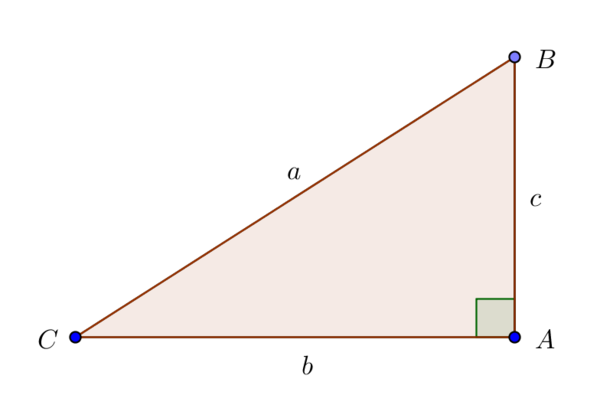
\includegraphics[width=.9\linewidth]{./fig/teorema-coseno-1.png}
\end{center}

\begin{align*}
a^2 &= b^2 + c^2
    && \text{Teorema de Pitágoras} \\
c^2 &= a^2 - b^2
    && \text{Despejando $c^{2}$}\\
    &= a^2 - 2 b^2 + b^2
    && \text{Sumando $0 = b^2 - b^2$ a la derecha} \\
    &= a^2 - 2 a b \left({\frac b a}\right) + b^2
    && \text{Multiplicando $2 b^2$ por $\dfrac a a$} \\
    &= a^2 + b^2 - 2 a b \cos C
    && \text{Por la definición de $\cos C = \dfrac b a$}
\end{align*}


\emph{Caso del triángulo acutángulo}

Sea \(\triangle ABC\) un triángulo acutángulo.

\begin{center}
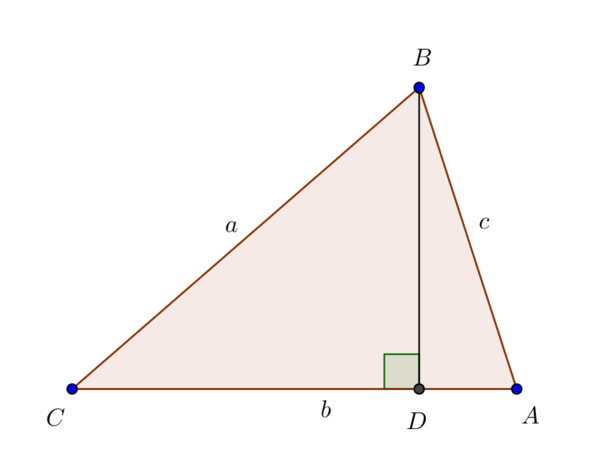
\includegraphics[width=.9\linewidth]{./fig/teorema-coseno.2.png}
\end{center}

Sea \(BD\) perpendicular a \(AC\) y se definen \(h = BD\), \(e = CD\) y \(f = AD\).

Los triángulos \(\triangle CDB\) y \(\triangle ADB\) son rectángulos. Por tanto, \\
\begin{align*}
c^2 &= h^2 + f^2
    && \text{Teorema de Pitágoras} \\
    &= a^2 - e^2 + f^2
    && \text{Teorema de Pitágoras} \\
    &= a^2 - e^2 + f^2 + 2e^2 - 2e^2 + 2ef - 2ef
    && \text{Sumando $2e^2 - 2e^2 + 2ef - 2ef$} \\
    &= a^2 + (e^2 + f^2 + 2ef) - 2e(e + f)
    && \text{Agrupando} \\
    &= a^2 + (e + f)^2 - 2e(e+f)
    && \text{Cuadrado del binomio} \\
    &= a^2 + b^2 - 2eb
    && \text{Sustituyendo $b = e + f$} \\
    &= a^2 + b^2 - 2 a b \cos C
    && \text{Definición de $\cos C = \frac{e}{a}$} \\
\end{align*}

\emph{Caso del triángulo obtusángulo}

Sea \(\triangle ABC\) un triángulo obtusángulo.

\begin{center}
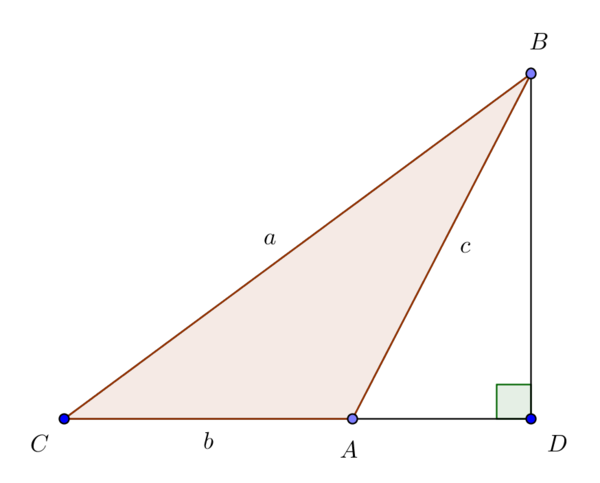
\includegraphics[width=.9\linewidth]{./fig/teorema-coseno-3.png}
\end{center}

Se extiende \(AC\) y sea \(BD\) perpendicular a \(AC\). Se define \(h = BD\), \(e = CD\) y \(f = AD\).

Entonces \(\triangle CDB\) y \(\triangle ADB\) son triángulos rectángulos. Por tanto,

  \begin{align*}
c^2 &= h^2 + f^2
    && \text{Teorema de Pitágoras} \\
    &= a^2 - e^2 + f^2
    && \text{Teorema de Pitágoras} \\
    &= a^2 - (b + f)^2 + f^2
    && \text{Por definición de $e$ y $f$} \\
    &= a^2 - b^2 - f^2 - 2bf + f^2
    && \text{Expandiendo el cuadrado del binomio} \\
    &= a^2 - b^2 - 2bf
    && \text{Cancelando $f^2 - f^2$} \\
    &= a^2 - b^2 - 2bf + 2b^2 - 2b^2
    && \text{Sumando y restando $2b^2$} \\
    &= a^2 + b^2 - 2b(b + f)
    && \text{Reagrupando} \\
    &= a^2 + b^2 - 2be \\
    &= a^2 + b^2 - 2 a b \cos C
    && \text{Por definición de $\cos C = \frac{e}{a}$}
  \end{align*}
\end{demostracion}

\item 129
\begin{teorema}
Teorema de Pitágoras: Sea \(\triangle ABC\) un triángulo rectángulo
\(c\) como su hipotenusa. Entonces,
$$a^2 + b^2 = c^2$$
\end{teorema}
\begin{demostracion}
\begin{align*}
c^2 &= a^2 + b^2 - 2 a b \cos\left(\frac{\pi}{2}\right) \\
    &= a^2 + b^2
\end{align*}
\end{demostracion}
\end{itemize}
\end{document}
